A common, simple and highly used building block for parallel algorithms is scan also know as all-prefix-sum. Scan calculates all partial reductions of a set, as defined by Blelloch \cite{BlellochTR90} in \cref{def:al_blelloch_scan}.

\begin{definition}
\label{def:al_blelloch_scan}
\textit{The scan operation takes a binary associative operator $\oplus$, and an ordered set of n elements}
\begin{center}
$[a_0,a_1,...,a_{n-1}],$
\end{center}
\textit{and returns the ordered set}
\begin{center}
$[a_0, (a_0 \oplus a_1),...,{a_0 \oplus a_1 \oplus ... \oplus a_{a_n-1}}].$
\end{center}
\end{definition} 
\begin{example}
\textit{For binary associative operator $+$, and the input set}
\begin{center}
	$[1,2,3,4,5,6,7,8],$
\end{center}
\textit{the return is}
\begin{center}
	$[1,3,6,10,15,21,28,36].$
\end{center}
\end{example}

The scan, like the reduction in \cref{sec:al_reduction}, is using the binary associative operator, and can therefore be used for e.g. addition or multiplication. There is distinguished between two types of scan, the exclusive scan also know as prescan and the inclusive scan. The inclusive scan is defined as \cref{def:al_blelloch_scan} where as exclusive scan is defined accordingly to Blelloch \cite{BlellochTR90} as \cref{def:al_blelloch_prescan}:

\begin{definition}
	\label{def:al_blelloch_prescan}
	\textit{The prescan operation takes a binary associative operator $\oplus$ with identity I, and an ordered set of n elements}
	\begin{center}
		$[a_0,a_1,...,a_{n-1}],$
	\end{center}
	\textit{and returns the ordered set}
	\begin{center}
		$[I,a_0, (a_0 \oplus a_1),...,{a_0 \oplus a_1 \oplus ... \oplus a_{a_n-2}}].$
	\end{center}
\end{definition}
\begin{example}
	\textit{For the binary associative operator $+$ with the identity $0$, and the input set}
	\begin{center}
		$[1,2,3,4,5,6,7,8],$
	\end{center}
	\textit{the return is}
	\begin{center}
		$[0,1,3,6,10,15,21,28].$
	\end{center}
\end{example}

Both types of scan can be acquired from one another by shifting. They are both used in different applications benefiting from there differences. Blelloch \cite{BlellochTR90} also describes the scan as a good example of an algorithm that seems inherently sequential, but for which there is an efficient parallel implementation. \Cref{fig:scan_serial} show a visual representation of the common serial implementation of the scan.  

\begin{figure}[ht]
	\centering
	\fbox{
		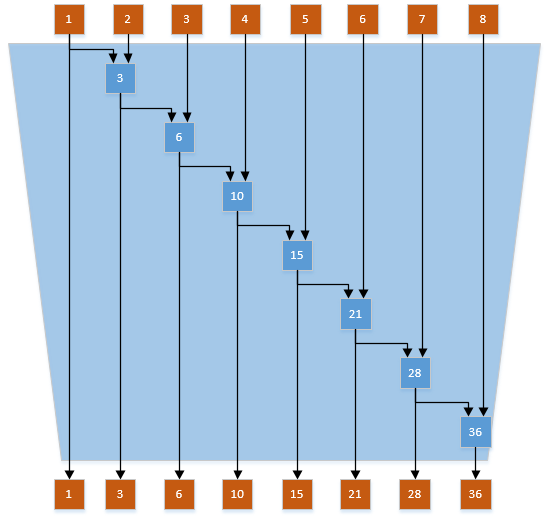
\includegraphics[width=0.5\textwidth]{figs/algorithm/scan_serial.png}}
	\caption{Serial implementation of Scan}
	\label{fig:scan_serial}
\end{figure}

The algorithm like the serial reduction on \cref{fig:reduce_serial}, but cannot be paralleled the same way because of the more strict chain of dependencies. Like the serial reduction, scan has a work and step complexity of $\mathcal{O}(n)$. The next two subsections will describe two different parallel implementations of the scan algorithm.